\SubCity{Saragar}
{30,000 (85\% humans, 6\% elves, 6\% dwarves, 2\% other)}
{Metal weapons, puddingfish cloth, fresh water}
{Saragarian}
{
\begin{figure}[b!]
\centering
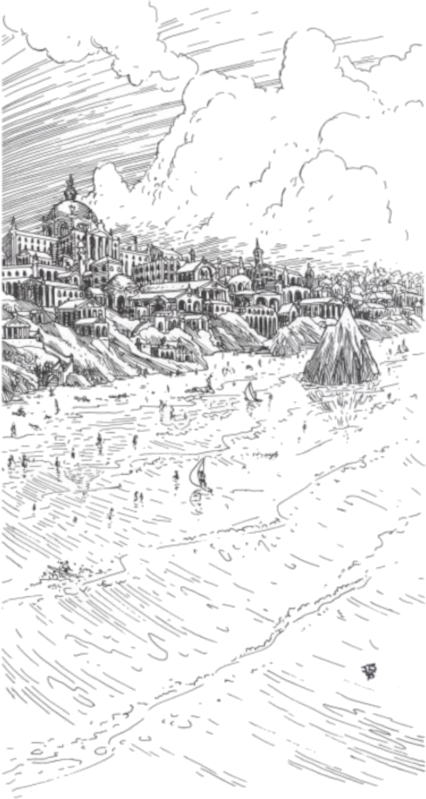
\includegraphics[width=\columnwidth]{images/saragar-1.png}
\end{figure}

	Separated from the rest of the region by the Burning Plains and the Thunder Mountains, the city of Saragar sits on the shores of the Last Sea, called Marnita by Saragarians. Visitors from the Tablelands would consider Saragar a miracle. All of the drudge work performed by slaves in other cities is taken care of by the minds of ancient criminals trapped forever in obsidian spheres. The streets are cleaned, cattle herded, crops tended, garbage removed, and water purified by these psionic powered spheres.

	The only price the citizens must pay to have all of their needs looked after in this way is that they must remain happy. The primary law of Saragar is, ``Happiness must be maintained!''
}
{
	For the most part Saragar maintains a closed self-sufficient society. To visit Saragar is to step back into the Green Age. People dress in tabards and gowns befitting a less savage age. The relatively cooler climate in the vale makes such clothing practical and comfortable. There is an abundance of metal in Saragar compared to the Tablelands, though most of it is ancient and shows signs of wear. Some new sources of ore exist in the surrounding mountains, but few citizens of Saragar still know how to extract it, let alone forge it into new items.

	Someone from the city-states of the Tyr region might consider Saragar to be a paradise. That certainly is the perception the Triune Mind Lords try to propagate. They generate laws to bolster the illusion of happiness and serenity but do nothing to truly address those concerns. The lawkeepers enforce these rules. For this reason the Saragar dwellers have learned to constantly display serene attitudes.

	There are no wizards of any sort in Saragar. Wizardry is considered evil and most citizens in Saragar who witness it don't have any idea what they are seeing. Psionics are the true power of the domain.
}
{
	The basic form of Saragar's government is a triune of 	lawmakers who write the city's laws, an army of lawkeepers to enforce the laws, and a bureaucracy of lawtenders to perform the administrative function.

	The trio that make up Saragar's Triune Mind Lords are powerful, ageless masters of psionics. They are Thesik (LE male mindlord human, kineticist 29), Barani (NE female mindlord human, telepath 28), and Kosveret (CE male mindlord elf, nomad 27). The citizens of Saragar consider the Mind Lords gods and treat them as such; thought there is little interaction between the Mind Lords and the populous.

	Senior Lawkeeper Efkenu (LN male human, psychic warrior 17) is the only person to have regular contact with the Mind Lords. He passes on their edicts and as head of the lawkeepers sees that their laws are enforced. Though a fair man, Efkenu makes no distinctions between the types of offenses and all criminal acts are punished in the same manner. The accused is taken to the harmonizers. The harmonizers are psions who reach into a subject's mind to sift and shape thoughts back to the track the Mind Lords have dictated.

	The lawkeepers are as corrupt as any templar. They enforce the laws arbitrarily and to suit their own desires. Supervisors rarely leave their offices to check on their subordinates and only rebuke subordinates for their behavior if it interferes with their own plans.

	The lawtenders perform all of the administrative work. They tend to be the most optimistic of people, determined that there is no problem that cannot be solved with a little determination and positive thinking. While they are not corrupt like the lawkeepers, the lawtenders are not very good administrators. They insist on only performing their duties by the book, and refuse to delineate from their guidelines no matter how inefficient or incorrect those guidelines are.
}
{
	\textbf{The Underground}: Despite the relative pleasantness of Saragar, there are some people who recognize that they are living in a society in decay; one that relies on powerful immortals for every aspect of their lives. These people make up the Underground which has been growing in Saragar for the past few hundred years.

	Most members of the Underground are just upset that their lives have become more inconvenient as some of the obsidian orbs have begun to fail. Others just like having someone to complain to without being arrested by the lawkeepers.

	A smaller group, who consider themselves the real Underground, speak out on street corners against the Mind Lords. They are always working on crazed schemes such as assassinating the Mind Lords, or destroying all of the obsidian orbs, but they lack the power to implement any of these plans.
}
{
	\textbf{Blufftown (Thorp, 50)}: This small settlement sits on the side of a bluff on an isolated butte in the middle of the Last Sea called the Lonely Butte. The lawkeepers generally refuse to set foot on the Lonely Butte unless directly ordered to do so by the Mind Lords, which makes Blufftown a perfect safe haven for the Underground and other fugitives from the Mind Lords' rule.

	The community is little more than a couple of inns sitting inside a cave in the side of a cliff. The only way to enter the village is to be hauled up in a device consisting of a large wicker basket and a series of ropes and pulleys powered by an obsidian orb.

	\textbf{Cubarto (Small Town, 1,500)}: Cubarto is located on the opposite of side of Marnita from Saragar. The people of Cubarto are loud and lusty and would not fit in Saragar. With the lack of a presence of the lawkeepers, most people in Cubarto support the Underground, though discreetly. The villagers make their living off of fishing and trade coming into their port on its way to Kharzden or Sylvandretta. The village is known throughout the valley of the Last Sea for throwing a large party at the end of the year at which a large public feast is held.

	\textbf{Kharzden (Large Town, 2,000)}: Kharzden is a Dwarven colony scattered through ancient mining shafts in the Thunder Mountains. Most of the veins of ore were mined out long ago, and most of the metal items the dwarves have are ancient. The Dwarven society is matriarchal and is lead by Queen Elakta. Her word is law and is to be obeyed by all. Queen Elakta refused to have much to do with the lawkeepers, and maintains the tradition in Kharzden of not calling for help from the lawkeepers. The dwarves live underground and grow subterranean crops in massive chambers underneath the mountains. The dwarves have always doubted the power of the Mind Lords to keep the rest of the world at bay, and tried to make their community as self sufficient as possible.

	\textbf{Shallat (Hamlet, 300)}: Shallat is one of a number of small fishing villagers on the shores of Marnita. What makes the village stand out is the Shallat family who rules the villages. Each member of the Shallat family is a skilled physician and many are also water clerics. The Shallat healers provide their services to anyone in need, no matter who they are. The villagers of Shallat are fun-loving people and are generally treated well by everyone living on the shores of the Last Sea. Even brigands and pirates do not harass the village, as potentially they might need the skills of the Shallat healers.

	\textbf{Sylvandretta (Small Village, 500)}: The elves of Sylvandretta are called ``ghost elves'' by the people of Saragar because of their fair skin and their cold and aloof nature. The ghost elves believe that the purity of their bloodline must be preserved above all other concerns, and isolate themselves from the other races of the Last Sea region.

	The secluded settlement of Sylvandretta is located in the Spirit Forest nestled within a grove of trees of life. The community is run by a council of seven elders, elected by the general Elven population.
}
{
	\textbf{The Distillery and the Water Tower}: The distillery is a psionically powered factory used to transform salt water from the Last Sea into fresh water. The water is pumped from the distillery into the water tower which is connected to a citywide plumbing network that pipes fresh water into every building in Saragar.

	\textbf{The Palace}: A massive palace overlooks the city of Saragar from a hill east of the city. Unlike the palaces of the sorcerer-kings, the palace of the Mind Lords was built more for awe-inspiring beauty than for defense. The security provided by the lawkeepers is lax around the palace, as the Mind Lords are confident they could handle any intruder.

	Statues of the three Mind Lords stand on a circular base at the highest point of the palace. The base slowly rotates throughout the day powered by an obsidian sphere. The people of Saragar use the statues to tell time, as the statues complete a full rotation every hour.
}
{
	\item Vikus and Mylandus are two merchants who run a successful business in Saragar until Mylandus disappears with most of the funds from the business. The PCs are hired by Vikus to track down his partner. Mylandus has discovered some secret that has scared him greatly enough that he has fled the city and is trying to leave the Last Sea area completely. Unfortunately for him, Mylandus has no idea how to survive in the devastated environment of the rest of Athas and will not survive long if he is able to find a way out of the area of the Last Sea.
	\item Jarsius, a tavern owner in Saragar, has begun to have disturbing visions, in which he sees himself behaving in random acts of violence. In actuality, the visions are memories. Jarsius was an active leader of the Underground until he was captured three years ago, but his memories were erased. The effect was not perfect and now some of his suppressed memories are returning. Members of the Underground still watch Jarsius, to see if he remembers what happened to him. For Jarsius's mind was not destroyed by the lawkeepers but by members of the Underground who acted to mindwipe him to protect their identities.
	\item The lawkeepers based at South Pass discover the tracks of a large beast they have never encountered before. The PCs, as outlanders who may have seen such a beast before, are drafted to help track down the beast.
	\item A wealthy Saragarian wants to see what the world is like outside of the Last Sea. He hires the PCs to get him through the Border of Guardians.
	\item Because of the ragged appearance of most outlanders, the PCs are mistaken for druids by a small fishing community. The villagers ask the PCs for help with a school of sharks that is making fishing difficult in the area.
	\item A man is found beaten to death. His face was so badly beaten that the only way to identify him was by a letter found in his pocket. The letter was addressed from one of the PCs, and the lawkeepers wish to talk to the PC to see how he was involved with the murdered man. The PC has never heard of the man and has no idea why the dead man had the PCs name in his pocket.
}